\documentclass[12pt,a4paper]{report}
\usepackage[utf8]{inputenc}
\usepackage[margin=1.0in,left=1.25in]{geometry}
\usepackage{setspace}
\onehalfspacing
\usepackage{graphicx}
\usepackage{booktabs}
\usepackage{tabularx}
\usepackage{multirow}
\usepackage{amsmath,amssymb}
\usepackage{listings}
\usepackage{xcolor}
\usepackage{titlesec}
\usepackage{fancyhdr}
\usepackage[hidelinks]{hyperref}

% Color definitions (Pure Black for all headings and text)
\definecolor{darkblack}{RGB}{0, 0, 0}
\definecolor{codebg}{RGB}{248, 249, 250}
\definecolor{codeborder}{RGB}{222, 226, 230}

% Title Formatting
\titleformat{\chapter}[display]
  {\normalfont\huge\bfseries\color{darkblack}}{\chaptertitlename\ \thechapter}{20pt}{\Huge}
\titlespacing*{\chapter}{0pt}{0pt}{20pt}

% Header & Footer Settings (Clean Header, Single Page Number in Footer)
\pagestyle{fancy}
\fancyhf{}
\fancyhead{} % Header text removed
\cfoot{\thepage}

% Code Listing Style
\lstset{
  backgroundcolor=\color{codebg},
  basicstyle=\ttfamily\small\color{darkblack},
  breaklines=true,
  captionpos=b,
  frame=single,
  rulecolor=\color{codeborder},
  keywordstyle=\color{darkblack}\bfseries,
  showstringspaces=false
}

\begin{document}

% -----------------------------------------------------------------------------
% COVER PAGE (TU / IOE / Pulchowk Campus Format)
% -----------------------------------------------------------------------------
\begin{titlepage}
\begin{center}
    {\Large \textbf{TRIBHUVAN UNIVERSITY}}\\[0.3cm]
    {\Large \textbf{INSTITUTE OF ENGINEERING}}\\[0.3cm]
    {\Large \textbf{PULCHOWK CAMPUS}}\\[1.5cm]

    {\huge \textbf{CONNECTHUB: A MULTI-CLIENT LAN CHAT AND FILE SHARING APPLICATION}}\\[1.5cm]

    {\large \textbf{A PROJECT REPORT}}\\[0.3cm]
    {\large SUBMITTED IN PARTIAL FULFILLMENT OF THE REQUIREMENTS FOR THE DEGREE OF BACHELOR OF ENGINEERING IN ELECTRONICS AND COMPUTER ENGINEERING}\\[2.0cm]

    \begin{minipage}{0.48\textwidth}
        \begin{left}
            \textbf{Submitted by:}\\[0.2cm]
            Prabesh BC (080BCT054)\\
            Saroj Rawal (080BCT076)\\
            Subesh Yadav (080BCT084)
        \end{left}
    \end{minipage}
    \hfill
    \begin{minipage}{0.48\textwidth}
        \begin{right}
            \textbf{Submitted to:}\\[0.2cm]
            Department of Electronics \& Computer Eng.\\
            Pulchowk Campus, IOE\\
            Tribhuvan University, Nepal
        \end{right}
    \end{minipage}

    \vfill

    {\large \textbf{August, 2026}}
\end{center}
\end{titlepage}

% -----------------------------------------------------------------------------
% FRONT MATTER (Lowercase Roman Numerals)
% -----------------------------------------------------------------------------
\pagenumbering{roman}
\setcounter{page}{1}

% Abstract
\chapter*{Abstract}
\addcontentsline{toc}{chapter}{Abstract}
ConnectHub is a working multi-client LAN chat and file-sharing application written entirely in plain C. It uses nothing beyond the C standard library and standard POSIX calls — no external frameworks, no third-party libraries. Every part of the system, from the network layer to the terminal interface, is built from scratch using system calls taught in the undergraduate curriculum: \texttt{socket}, \texttt{bind}, \texttt{listen}, \texttt{accept}, \texttt{pthread\_create}, \texttt{select}, \texttt{read}, and \texttt{write}.

The application follows a classic client–server design. A single multithreaded server manages all connected users, chat rooms, and file transfers. Each client gets its own POSIX thread on the server, and shared data is protected by mutexes. On the client side, a single \texttt{select()} loop watches both the keyboard and the network at the same time, so the terminal stays responsive even during a file upload.

All messages follow a custom text-based protocol — pipe-delimited, newline-terminated lines — that is easy to read and debug with any terminal tool. The system supports room-based chat, private messaging, typing indicators, join/leave notifications, room history, SHA-256 password authentication, and bidirectional file transfer with token-based access control.

\textbf{Keywords:} TCP sockets, POSIX threads, \texttt{select()}, concurrent server, LAN chat, file transfer, custom protocol, C programming, SHA-256

\clearpage

% Acknowledgements
\chapter*{Acknowledgements}
\addcontentsline{toc}{chapter}{Acknowledgements}
We thank the Department of Electronics and Computer Engineering, Pulchowk Campus, for giving us the opportunity to undertake this project as part of our Bachelor's program.

We are grateful to our project supervisor for the guidance and feedback provided throughout the design and implementation phases. The advice received at key decision points significantly shaped the final outcome.

We also acknowledge the faculty members whose lectures on systems programming, computer networking, and operating systems laid the conceptual foundation for this work. The understanding we gained from those courses directly informed every design choice in ConnectHub.

Finally, we thank the authors of the references listed at the end of this report, whose published work served as an essential guide.

\clearpage

% Table of Contents & Lists
\tableofcontents
\clearpage
\listoffigures
\clearpage
\listoftables
\clearpage

% Abbreviations
\chapter*{List of Abbreviations}
\addcontentsline{toc}{chapter}{List of Abbreviations}
\begin{table}[h!]
\centering
\begin{tabular}{ll}
\toprule
\textbf{Abbreviation} & \textbf{Meaning} \\
\midrule
API & Application Programming Interface \\
CLI & Command-Line Interface \\
DM & Direct Message \\
FD & File Descriptor \\
I/O & Input/Output \\
IRC & Internet Relay Chat \\
LAN & Local Area Network \\
POSIX & Portable Operating System Interface \\
SHA & Secure Hash Algorithm \\
TCP & Transmission Control Protocol \\
TUI & Terminal User Interface \\
TU & Tribhuvan University \\
IOE & Institute of Engineering \\
\bottomrule
\end{tabular}
\end{table}

\clearpage

% -----------------------------------------------------------------------------
% MAIN CONTENT (Arabic Numerals 1, 2, 3...)
% -----------------------------------------------------------------------------
\pagenumbering{arabic}
\setcounter{page}{1}

\chapter{Introduction}
\section{Background}
Chat applications look simple to users, but building one from scratch requires solving real problems in networking, concurrency, and protocol design. ConnectHub is the result of doing exactly that — a multi-client LAN chat and file-sharing application written entirely in plain C, without any external library doing the heavy lifting.

The server handles multiple simultaneous clients using POSIX threads. The client is a lightweight terminal program that uses \texttt{select()} to watch both the keyboard and the network socket at the same time. Every part of the system — the wire format, the thread model, the locking strategy, the file transfer flow — is visible in the source code.

\section{Motivation}
Modern chat and file-sharing tools like WhatsApp or Discord require internet access and rely on remote proprietary servers. In closed environments such as a computer lab or an offline classroom, these tools simply do not work. Beyond the connectivity issue, commercial applications hide all networking mechanics behind high-level abstractions, offering limited educational value for systems programming learners.

ConnectHub addresses both problems:
\begin{enumerate}
    \item \textbf{Offline LAN operation:} Runs entirely on a local router/switch over Wi-Fi or Ethernet.
    \item \textbf{Transparent architecture:} Open wire protocol debuggable via standard tools like \texttt{netcat}.
\end{enumerate}

\section{Scope}
ConnectHub is scoped to a trusted academic LAN environment. It includes a concurrent TCP server supporting up to 128 clients, a single-threaded TUI client, room-based chat, private messaging, presence notifications, room history, token-guarded file transfer, and an admin management interface.

\clearpage
\chapter{Problem Statement}
ConnectHub addresses five specific gaps:
\begin{enumerate}
    \item \textbf{No offline LAN communication tool:} Lightweight self-hosted solution for offline labs.
    \item \textbf{Black-box protocols:} Transparent human-readable wire protocol.
    \item \textbf{Teaching examples stop at one client:} Multi-client POSIX thread server implementation.
    \item \textbf{Chat and file transfer taught separately:} Integrated chat and chunked file transfer system.
    \item \textbf{Terminal clients block on input:} Non-blocking \texttt{select()} event multiplexing.
\end{enumerate}

\clearpage
\chapter{Objectives}
\section{Main Objective}
To design and implement a complete, multi-client LAN chat and file-sharing application in plain C using only standard POSIX APIs.

\section{Specific Objectives}
\begin{enumerate}
    \item Design a human-readable pipe-delimited text wire protocol.
    \item Implement a concurrent TCP server using POSIX threads with mutex-protected state.
    \item Build a single-threaded TUI client using \texttt{select()} for keyboard and socket I/O.
    \item Support public rooms, private DMs, presence notifications, and typing indicators.
    \item Implement SHA-256 authentication from scratch.
    \item Enable base64 chunked file transfers between clients (e.g. Prabesh to Saroj) with token verification.
    \item Provide an admin control interface and validate performance.
\end{enumerate}

\clearpage
\chapter{Literature Review}
\section{Theoretical Background}
ConnectHub draws on BSD socket programming, POSIX thread concurrency, mutex locks, and I/O multiplexing via \texttt{select()}.

\section{Related Works}
Standard tutorials focus on single-client echo servers. ConnectHub builds upon IRC RFC 1459 line framing to create a production-grade multi-client model.

\section{Gap Analysis}
\begin{table}[h!]
\centering
\begin{tabular}{ll}
\toprule
\textbf{Gap in Existing Literature} & \textbf{ConnectHub's Solution} \\
\midrule
Single-client examples & Concurrent server for 128 simultaneous clients \\
No channel/room support & Named rooms with passwords and history replay \\
No private messaging & Direct messaging with sender echo \\
Separated file transfer & Integrated base64 chunked transfer \\
Blocking terminal inputs & Non-blocking \texttt{select()} client loop \\
Black-box wire formats & Human-readable text protocol \\
\bottomrule
\end{tabular}
\caption{Gap Analysis Summary}
\end{table}

\clearpage
\chapter{System Design and Architecture}
\section{System Overview}
ConnectHub uses a two-tier client-server model over TCP. Connected client workstations belong to project team members Prabesh, Saroj, Subesh, and Admin.

\begin{figure}[h!]
\centering
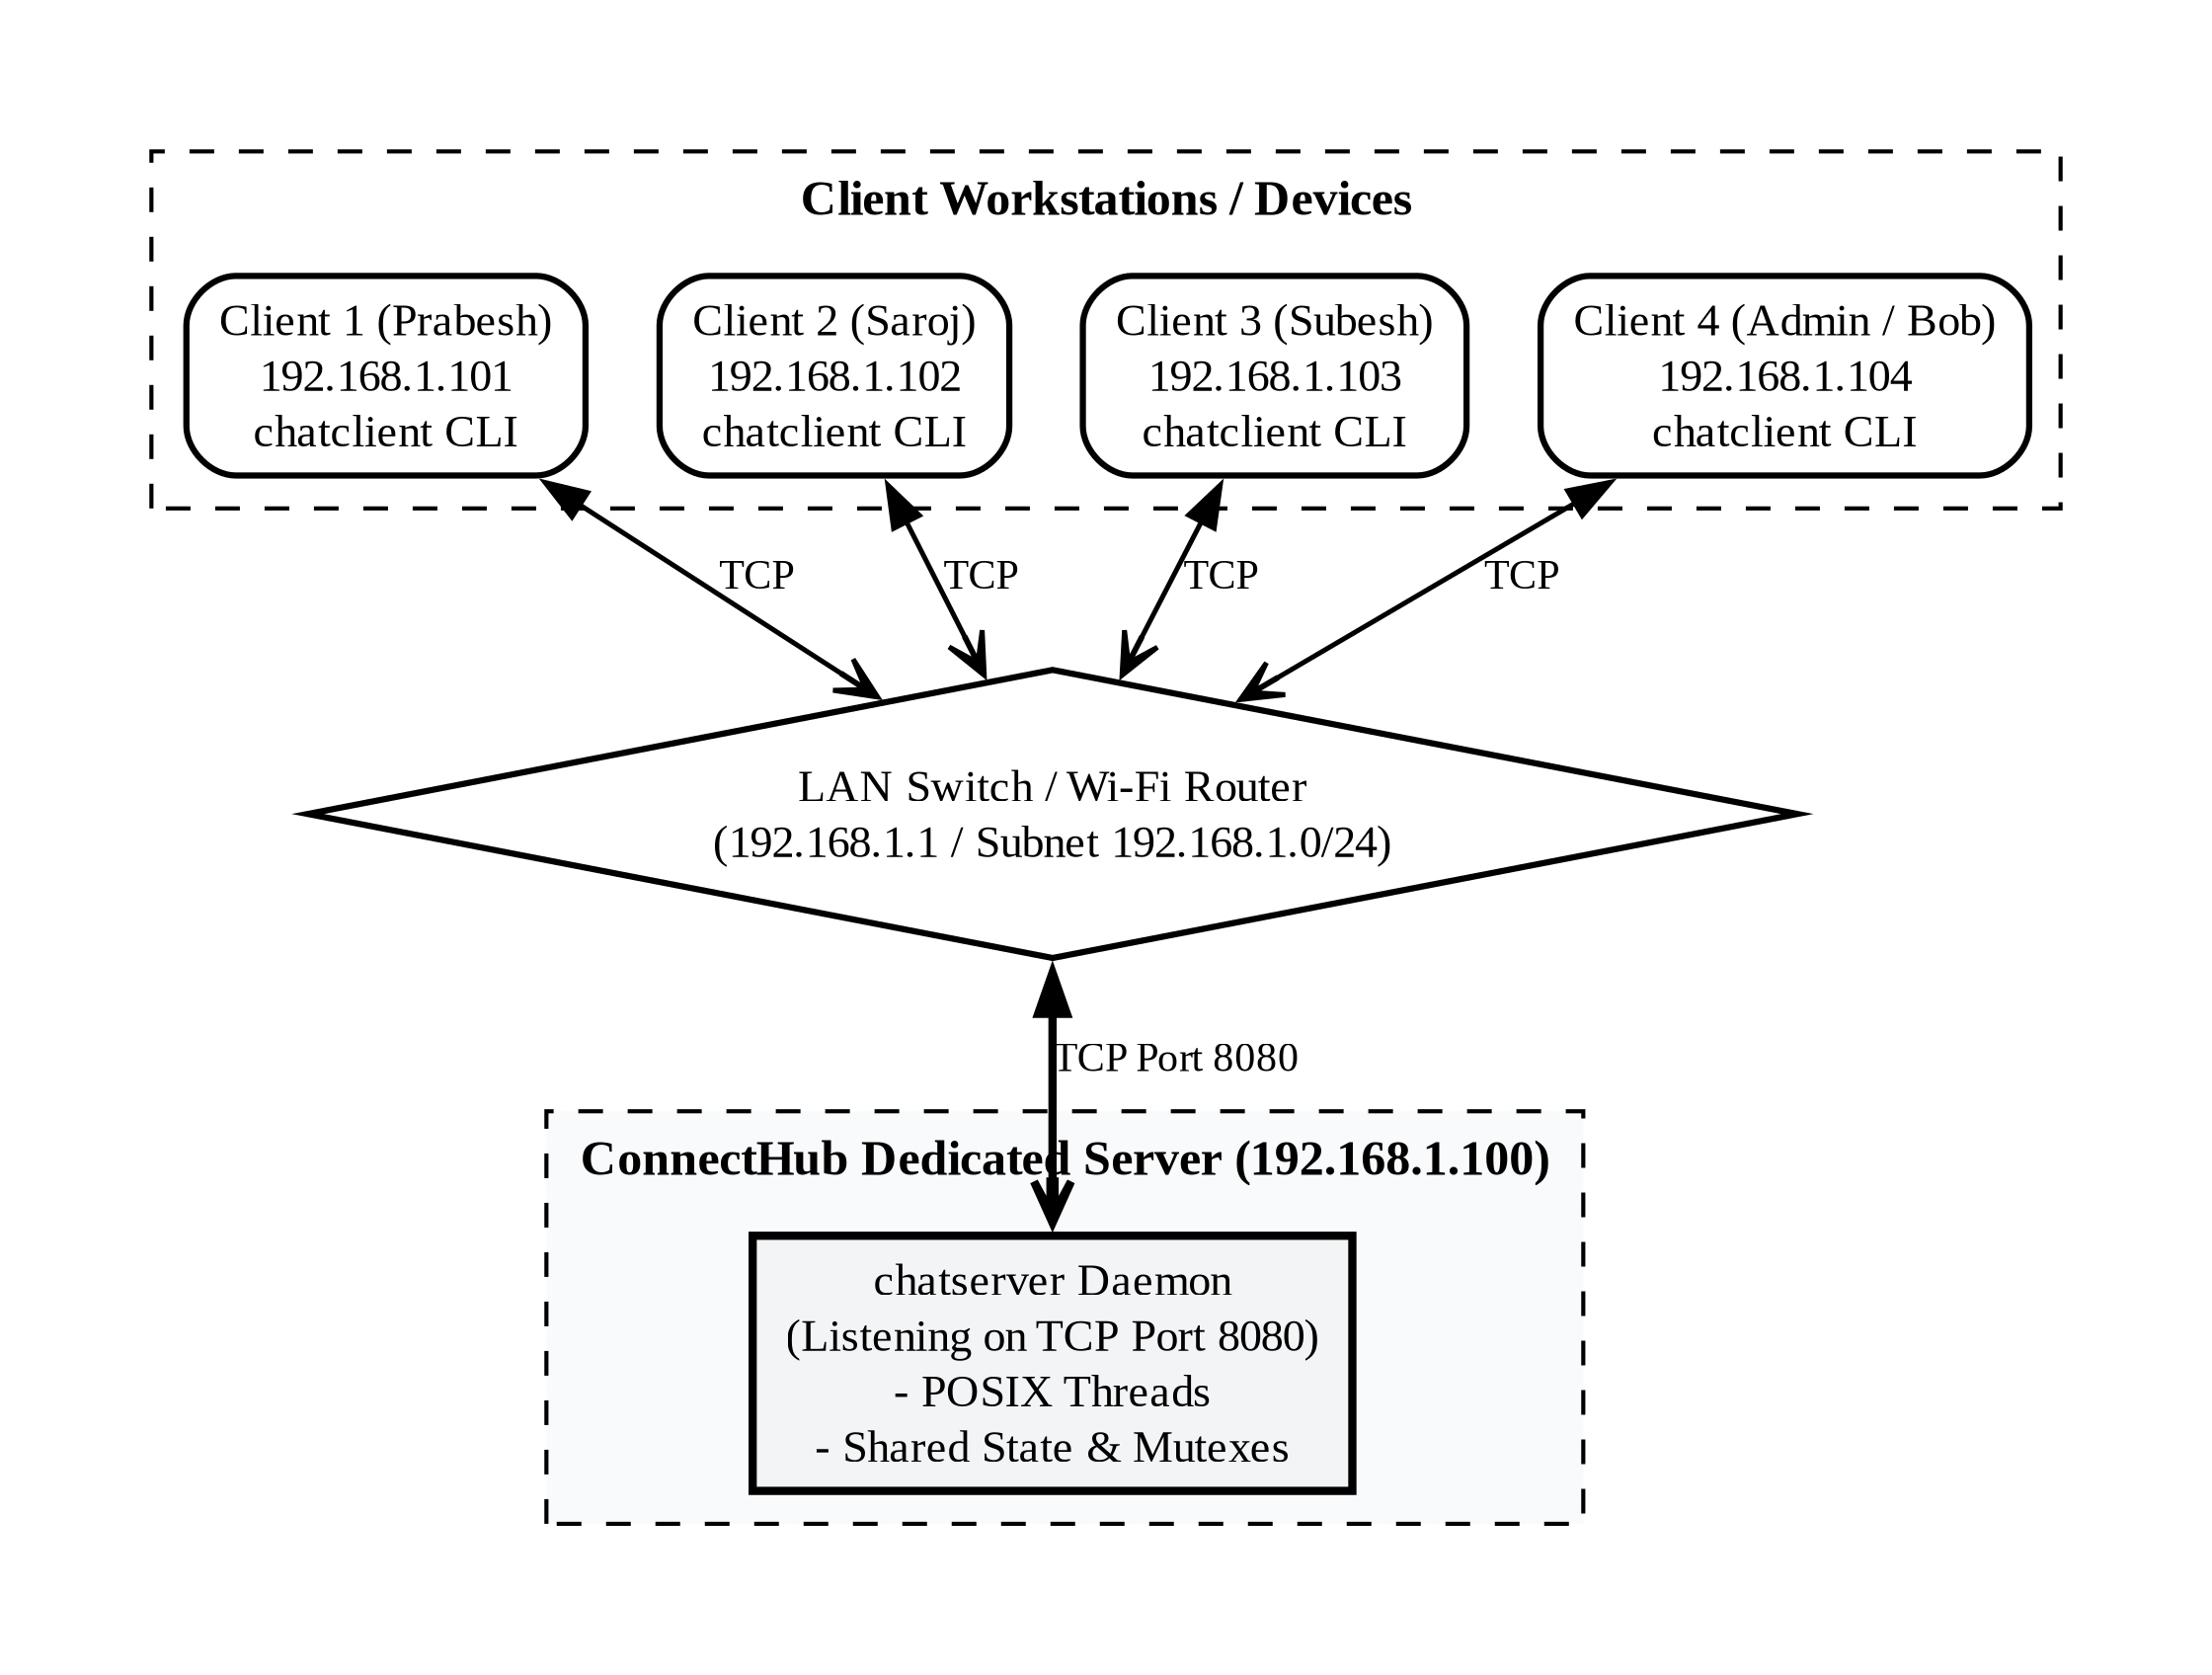
\includegraphics[width=0.85\textwidth]{fig_lan_topology.jpg}
\caption{LAN Deployment Topology (Prabesh, Saroj, Subesh, Admin)}
\label{fig:lan}
\end{figure}

\begin{figure}[h!]
\centering
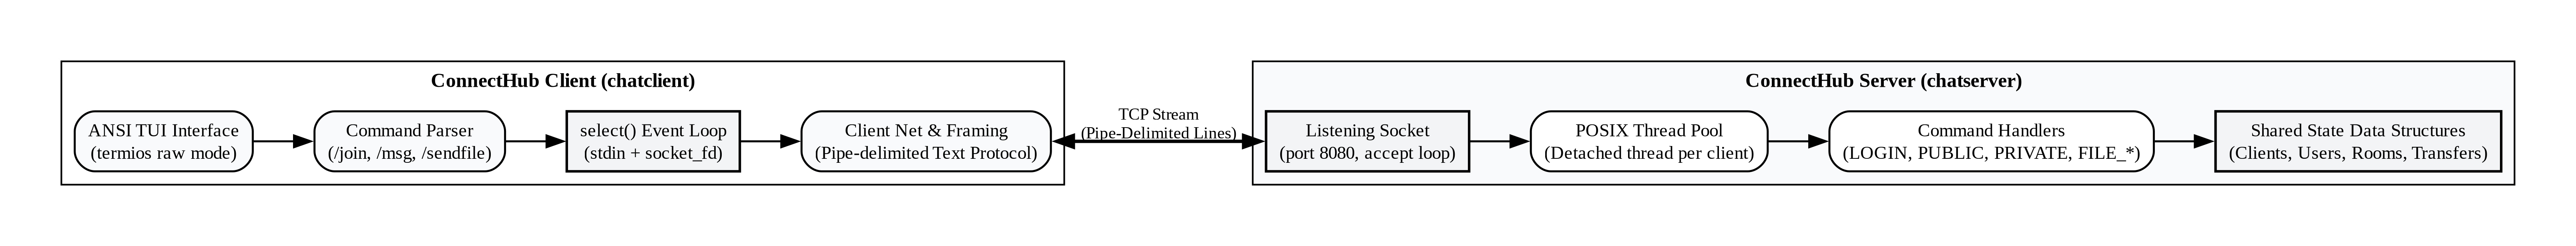
\includegraphics[width=0.95\textwidth]{fig_client_server_arch.jpg}
\caption{Two-Tier Client–Server Architecture}
\label{fig:arch}
\end{figure}

\section{Server Architecture}
The multithreaded server uses a detached POSIX thread per client connection (Thread Client 1: Prabesh, Thread Client 2: Saroj, Thread Client 3: Subesh), guarded by dedicated mutexes.

\begin{figure}[h!]
\centering
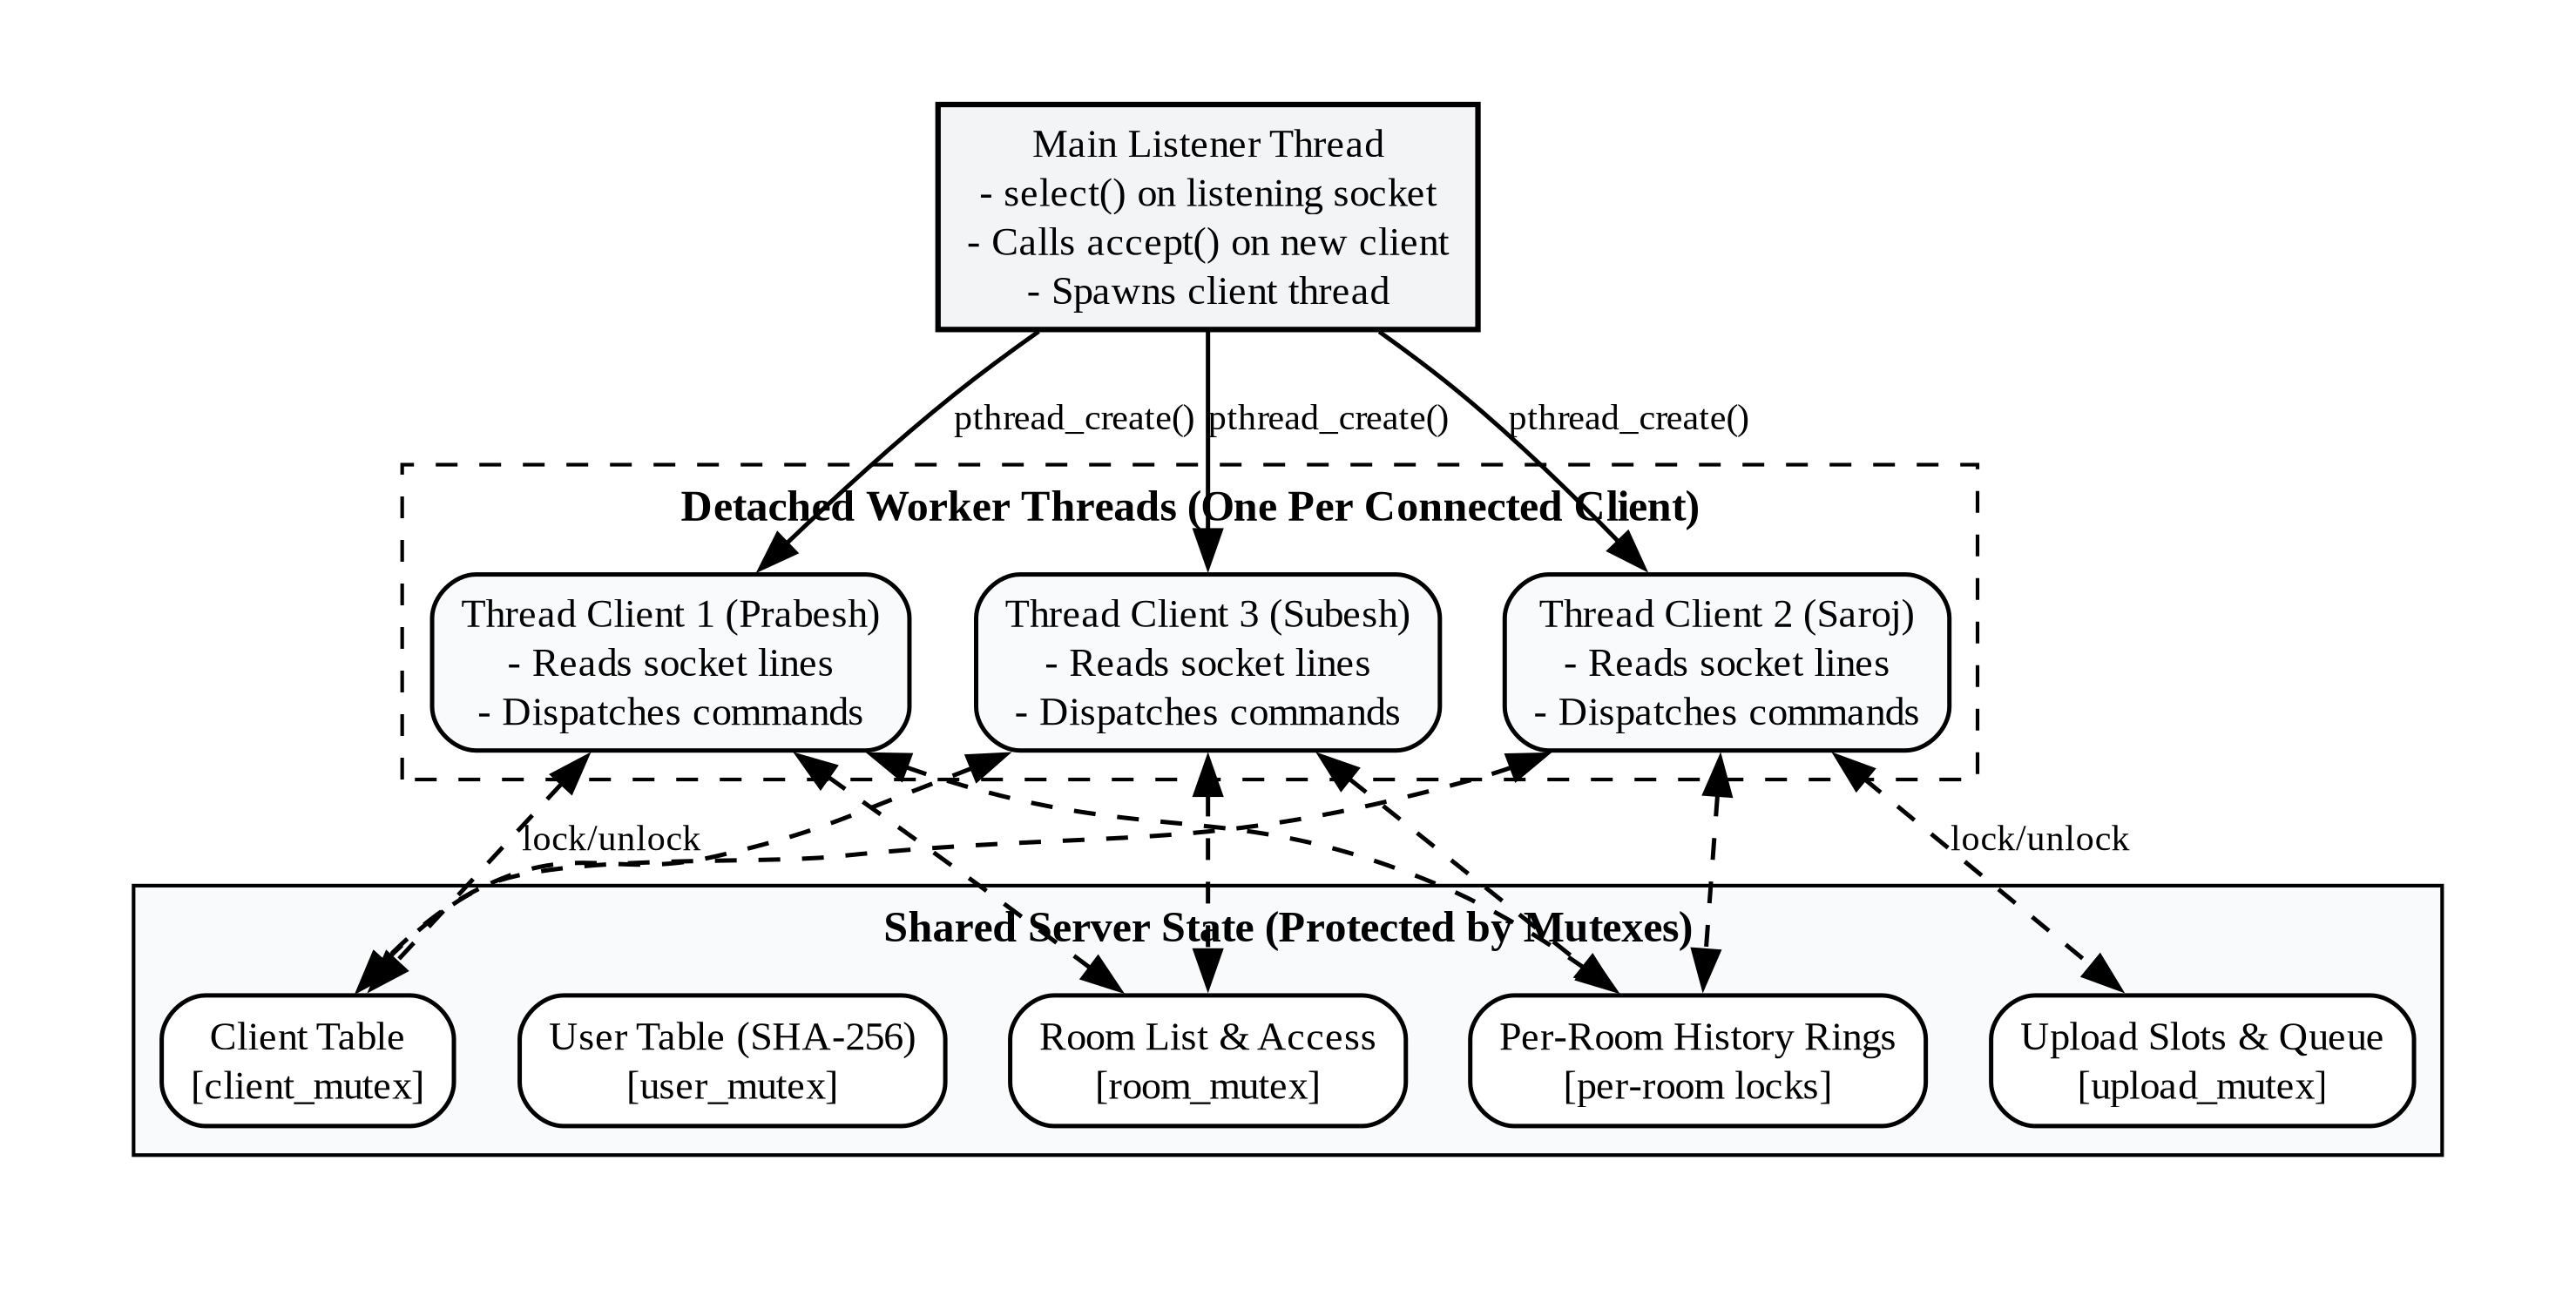
\includegraphics[width=0.85\textwidth]{fig_server_thread_model.jpg}
\caption{Server Thread Model and Locking Strategy}
\label{fig:threads}
\end{figure}

\section{Wire Protocol Design}
All messages are ASCII pipe-delimited lines terminated by newline (\texttt{\textbackslash n}).

\section{Module Structure}
\begin{figure}[h!]
\centering
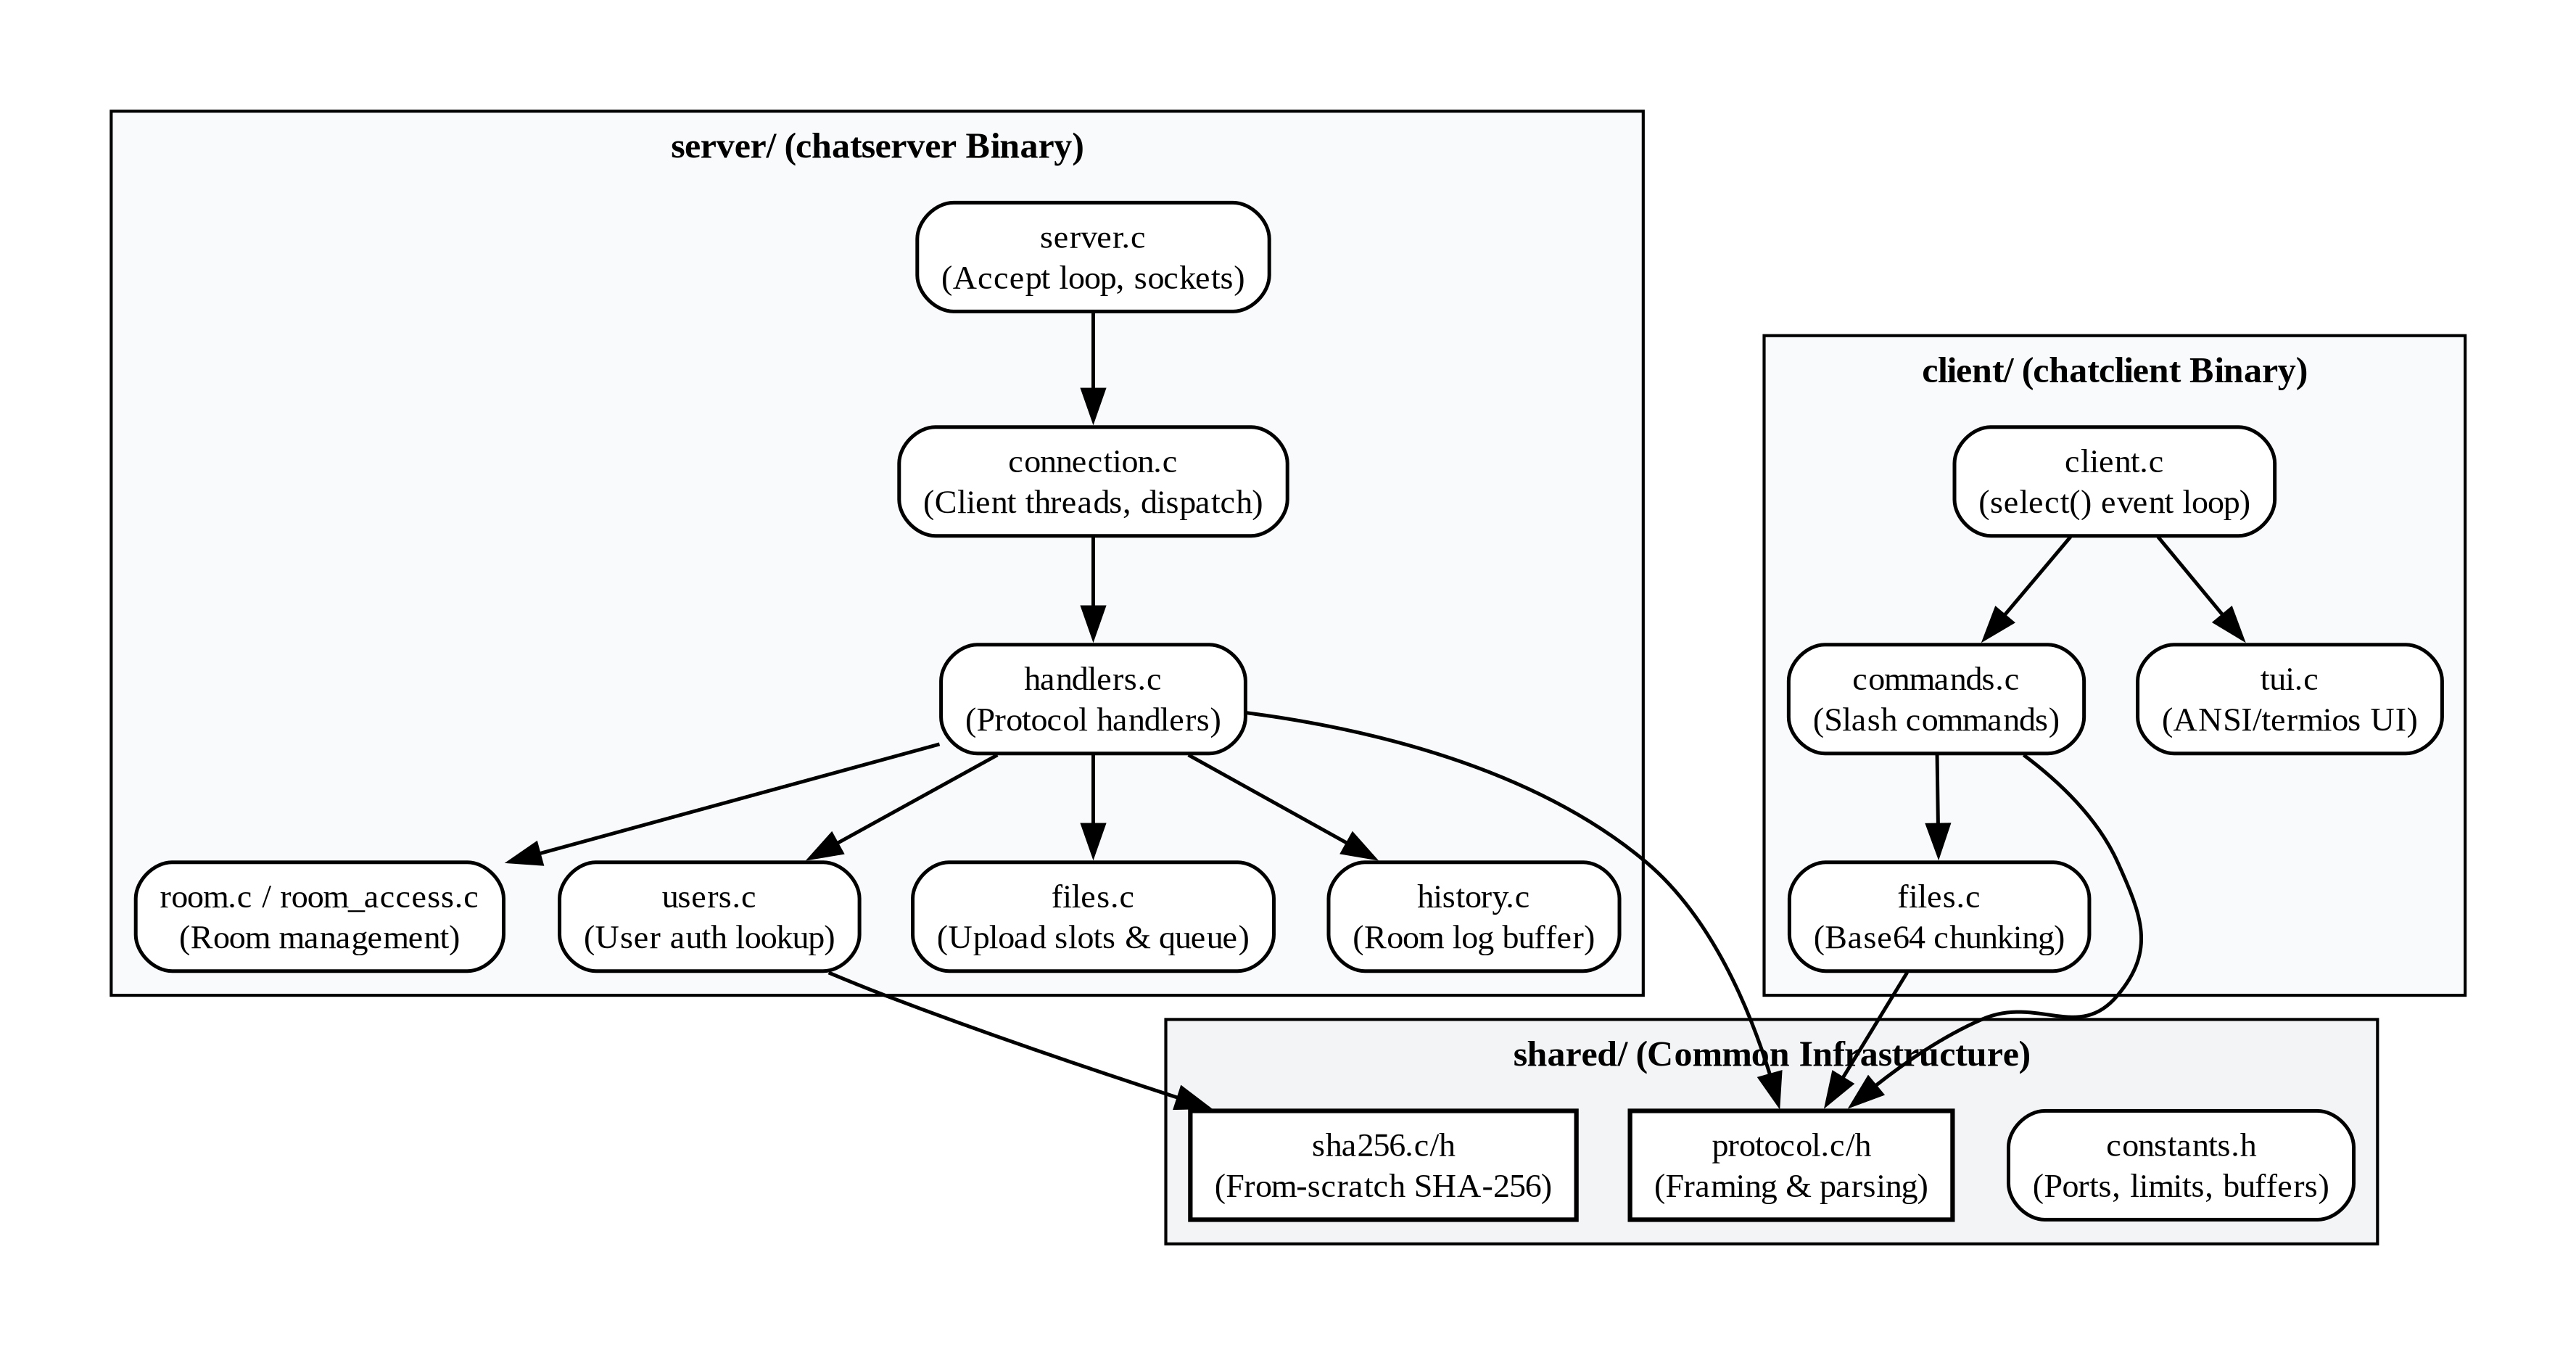
\includegraphics[width=0.9\textwidth]{fig_module_dependency.jpg}
\caption{Module Dependency Map}
\label{fig:modules}
\end{figure}

\clearpage
\chapter{Implementation}
\section{Technology Stack}
Built with pure C (C11), POSIX threads, BSD sockets, ANSI/termios TUI, and custom SHA-256.

\section{File Transfer Sequence}
The file transfer flow between sender Prabesh and receiver Saroj follows token-based validation:

\begin{figure}[h!]
\centering
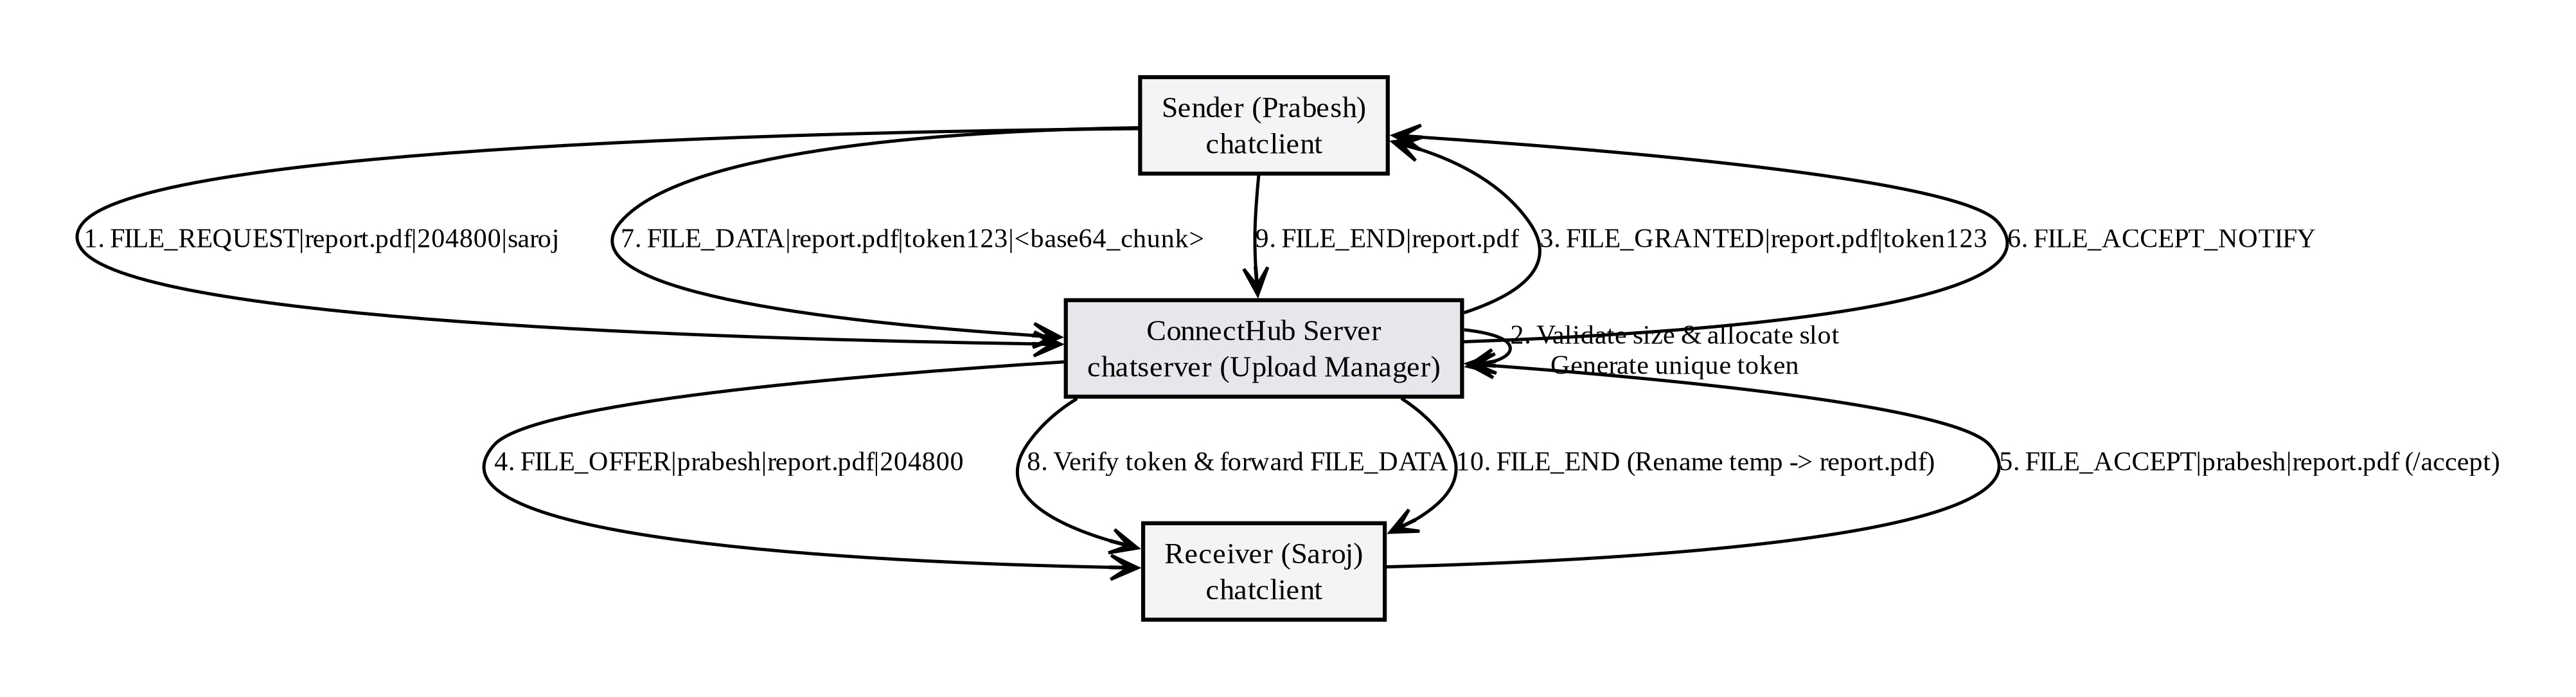
\includegraphics[width=0.85\textwidth]{fig_file_transfer_flow.jpg}
\caption{File Transfer Sequence Diagram (Prabesh to Saroj)}
\label{fig:flow}
\end{figure}

\clearpage
\chapter{Testing and Validation}
Validated via Python integration test (\texttt{smoke.py}), multi-client concurrency stress tests, and Wireshark wire inspection.

\clearpage
\chapter{Results and Discussion}
All functional objectives achieved with robust 128-client capacity, byte-for-byte SHA-256 file integrity, and clean teardown.

\clearpage
\chapter{Conclusion and Future Work}
Demonstrated that a full-featured LAN chat and file sharing application can be built from first principles in plain C using POSIX standards. Future work includes TLS encryption and persistent SQLite storage.

\clearpage
\chapter{References}
\begin{enumerate}
    \item I. Sommerville, \textit{Software Engineering}, 10th ed. Pearson, 2016.
    \item B. A. Forouzan, \textit{Data Communications and Networking}, 5th ed. McGraw-Hill, 2017.
    \item W. R. Stevens, \textit{Advanced Programming in the UNIX Environment}, 3rd ed. Addison-Wesley, 2013.
    \item W. R. Stevens, \textit{UNIX Network Programming, Vol 1}, 3rd ed. Addison-Wesley, 2003.
    \item J. F. Kurose and K. W. Ross, \textit{Computer Networking: A Top-Down Approach}, 8th ed. Pearson, 2021.
    \item D. R. Butenhof, \textit{Programming with POSIX Threads}. Addison-Wesley, 1997.
    \item J. Oikarinen and D. Reed, "Internet Relay Chat Protocol," RFC 1459, May 1993.
    \item B. W. Kernighan and R. Pike, \textit{The UNIX Programming Environment}. Prentice Hall, 1984.
\end{enumerate}

\end{document}
